\subsection{Benchmarking} %Correlating Microarchitecture with Performance\jled{change to ``Benchmarking''?}}
\label{sec:benchmark}


We design a microbenchmark suite to explore NVIDIA GPU microarchitecture features.
% Our following observations are drawn from analyzing the execution time of the microbenchmarks.
As shown in Figure~\ref{fig:workflow}, the CUDA kernel code is written in assembly and compiled into {\tt cubin} by our assembler, and then executed by CUDA APIs.
A CUDA kernel code is tested for hundreds of times, and the average time is used for accuracy.
The assembly instructions inside CUDA kernel are replicated to cover the branch overhead while not exceeding L1 instruction cache size.
%All assembly kernel codes are designed small enough to fit into the L1 instruction cache.
Timing ticks are recorded by {\tt S2R R0, SR\_CLOCKLO} instruction, in which
{\tt S2R} moves the value from the special clock register {\tt SR\_CLOCKLO} to a general
purpose register. 
Time is calculated in the general register and then written into the global memory.
%We run each benchmark program twice, disregarding the first run to avoid compulsory instruction cache misses.
Two metrics are benchmarked: latency and throughput. 
Latency is tested by a succession of \emph{dependent} instructions by launching only one thread block with $32$ threads/block, according to~\cite{fog}. 
Throughput is tested by a succession of \emph{independent} instructions by launching enough
threads (e.g. $26$ threads blocks with $512$ threads/block for Kepler) to make full use of CUDA cores and memory bandwidth.
%We use similar testing method with Fog's in~\cite{fog}.

% we tune the assembly codes of our microbench- marks using our assembler.
In this benchmarking process, we correlate microarchitecture features with the benchmark performance and get some meaningful observations in four microarchitecture features: register bank, 
control code, arithmetic throughput, and memory operation. 
These observations are useful to optimize program snippets of real-world applications.


\begin{figure*}
    \begin{subfigure}[htbp]{0.3\textwidth}
        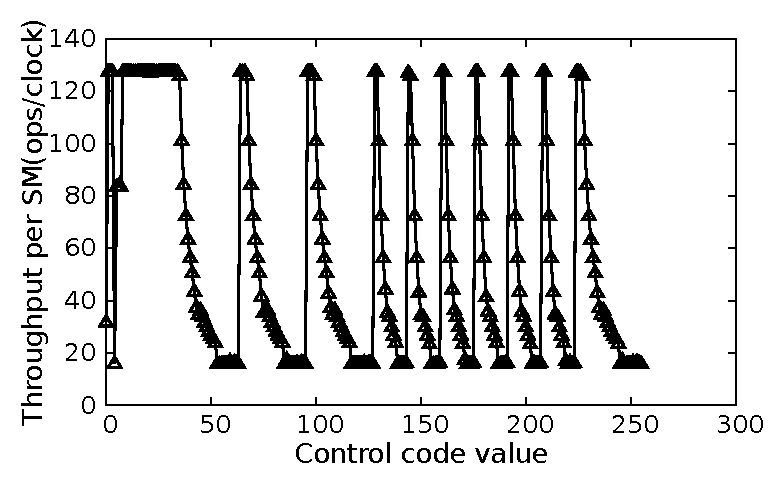
\includegraphics[width=2.1in]{ctrl}
        %\subcaption{Control code regulates {\tt FFMA} throughput.} %\jled{8-bit control code value} \jled{ops/cycle? or IPC?}}
        \subcaption{}
        \label{fig:control_throughput}
    \end{subfigure}
    \begin{subfigure}[htbp]{0.3\textwidth}
        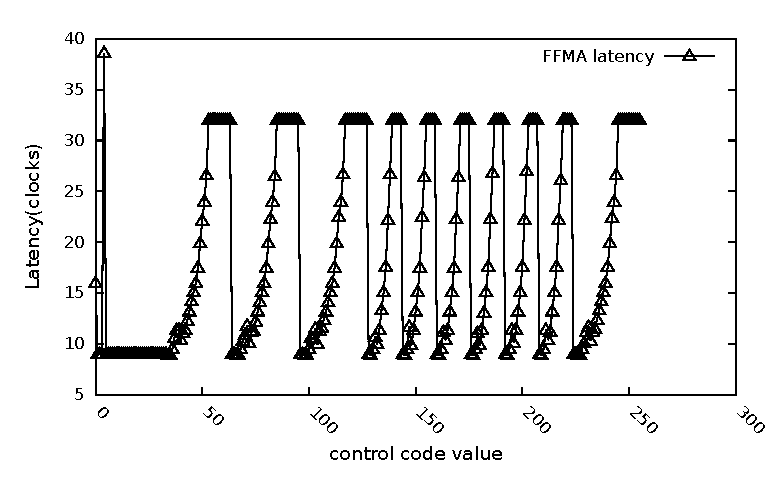
\includegraphics[width=2.1in]{ctrl_latency}
        \subcaption{}
        %\subcaption{Control code regulates {\tt FFMA} latency.} %\jled{8-bit control code value}}
        \label{fig:control_latency}
    \end{subfigure}
    \begin{subfigure}[htbp]{0.3\textwidth}
        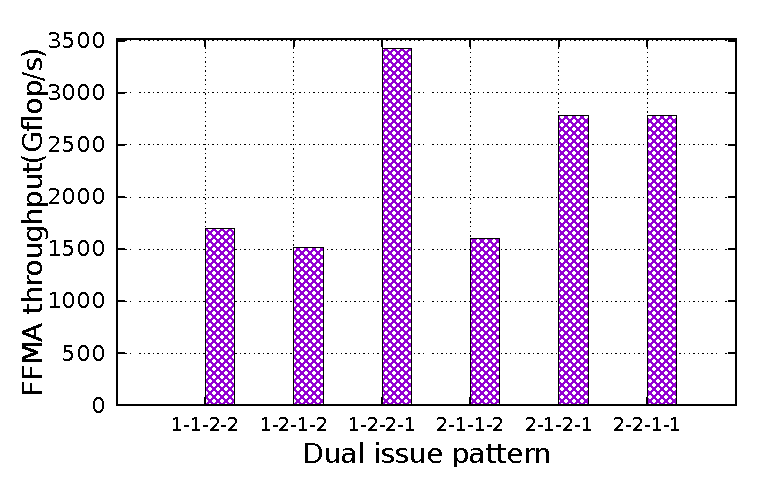
\includegraphics[width=2.1in]{pattern}
        \subcaption{}
        %\subcaption{Peak {\tt FFMA} throughput(1: single issue, 2: dual issue).}%\jled{Y-axis is performance?}}
        \label{fig:control_pattern}
    \end{subfigure}
    \caption{Different control code impact on performance(subfigure(\subref{fig:control_pattern}), 1$\rightarrow$single
    issue, 2$\rightarrow$dual issue).}
    \label{fig:control_code}
\end{figure*}


{\em {\bf Observation 1--[Register Bank]}:
Source registers may cause register bank conflicts that degrade instruction throughput.}

Shared memory bank conflicts are well-known as an important performance factor for CUDA programming.
Recent research~\cite{lai} has noticed that register bank conflicts are also innegligible.
To probe register bank distribution, our microbenchmarks measure the instruction throughput for different combinations of {\tt FFMA} register operands.
Table~\ref{tab:th} shows that different register combinations result in various efficiency and throughput.
The rightmost column represents the number of register bank conflicts recorded from our experiments.
This experiment is conducted in single issue mode by setting control code to 0x20.
Theoretically, without dual issue, the peak efficiency is $4\times32/192=66.67\%$, in which $4$ is the number of warp schedulers and $32$
is the number of threads in a warp.
In fact, we observe that both single- and dual-issue mode produce the same throughput behavior for bank conflicts.
 % variance of instruction throughput.
From our experiments on Kepler architecture, we observe:
\begin{itemize}
\item The destination registers do not contribute to bank conflicts, so they are free to be assigned to any bank.% no matter which bank is assigned to.
\item When source registers have 2-way or 3-way register bank conflicts, the throughput of float instructions will drop by 2.33\% and 17.17\% respectively in the single-issue mode.
\item A proper register distribution is found through benchmarking to eliminate bank conflict.
     Table~\ref{tab:reg} lists partial registers and their corresponding banks for NVIDIA Tesla K20m, which is consistent with GTX680~\cite{lai}, though K20m is different from GTX680 in maximal number of registers per thread and instruction encodings.
        %\\
% bank0$\Leftarrow$($Ridx \% 8 < 4$ \&\& $Ridx \% 2 == 0$) \\
% bank2$\Leftarrow$($Ridx \% 8 < 4$ \&\& $Ridx \% 2 == 1$) \\
%bank1$\Leftarrow$($Ridx \% 8 > 4$ \&\& $Ridx \%2 == 0$) \\
%bank3$\Leftarrow$($Ridx \% 8 < 4$ \&\& $Ridx\% 2 == 1$)\\
%where $Ridx$ is the register number.
%This rule will guide the performance tuning of SGEMM code.

\end{itemize}


\begin{table}[htbp]
    \caption{The efficiency of instruction throughput varies with different register combinations.Inst: instruction patterns, Th/SM: instruction throughput per SM, Eff: throughput efficiency,  Conf: register bank conflicts.}
\centering
\scalebox{0.8} {
\begin{tabular}{|c|c|c|c|}
\hline
Inst &Th/SM&Eff&Conf\\
\hline
{\tt FFMA R5,R4,R1,R0}&127.50&66.40\%&0\\
\hline
{\tt FFMA R2,R4,R1,R0}&127.50&66.40\%&0\\
\hline
{\tt FFMA R5,R2,R1,R0}&119.18&62.07\%&2-way\\
\hline
{\tt FFMA R3,R2,R1,R0}&119.18&62.07\%&2-way\\
\hline
{\tt FFMA R5,R9,R3,R1}&94.52&49.23\%&3-way\\
\hline
{\tt FFMA R11,R9,R3,R1}&94.52&49.23\%&3-way\\
\hline
{\tt FMUL R4,R1,R0}&127.50&66.40\%&0\\
\hline
{\tt FMUL R4,R2,R0}&119.17&62.06\%&2-way\\
\hline
\end{tabular}
}
\label{tab:th}
\end{table}


\begin{table}[htbp]
\caption{Partial register bank distribution.}
\centering
\scalebox{0.8} {
\begin{tabular}{|c|c|c|c|c|c|c|c|c|}
\hline
    {\tt Bank0}&{\tt R0}&{\tt R2}&{\tt R8}&{\tt R10}&{\tt R16}&{\tt R18}&{\tt R24}&{\tt R26}\\
\hline
    {\tt Bank1}&{\tt R1}&{\tt R3}&{\tt R9}&{\tt R11}&{\tt R17}&{\tt R19}&{\tt R25}&{\tt R27} \\
\hline
    {\tt Bank2}&{\tt R4}&{\tt R6}&{\tt R12}&{\tt R14}&{\tt R20}&{\tt R22}&{\tt R28}&{\tt R30}\\
\hline
    {\tt Bank3}&{\tt R5}&{\tt R7}&{\tt R13}&{\tt R15}&{\tt R21}&{\tt R23}&{\tt R29}&{\tt R31}\\
\hline
\end{tabular}
}
\label{tab:reg}
\end{table}



{\em {\bf Observation 2--[Control Code]}:
Warp scheduling and issue mode are tunable by modifying control codes which regulate instruction issue.}

Starting with the Kepler architecture, NVIDIA has been moving some control logics off the chip and into kernel
instructions to save power~\cite{lai,maxas}. 
This evolution provides programmers the opportunity to
make globally optimal scheduling decisions and other control optimizations if an assembler is available. 
 % and cuBLAS library
The disassembly codes from sample programs indicate that a $64$-bit binary control code controls $7$ instructions as Figure~\ref{fig:assemblycode} shows.
% a control code is placed before $7$ instructions, and it
We identify that the highest $6$ bits and the lowest $2$ bits are the {\em opcode} field of the scheduling instructions, and the middle $56$ bits are used to control the execution of the following $7$ instructions, each of which is assigned to a $8$-bit control code.


% statically examining the disassembly codes of cuBLAS and
We figure out the control code meanings by benchmarking instruction sequences of different control codes.
Bits-$4, 5, 7$ represent shared memory, global memory, and texture cache dependency barrier respectively.
% bit-$5$ represents global memory dependency
% barrier, and bit-$7$ indicates a texture cache dependency barrier. % due to its weak consistency cache model.
%Unexpected values will be loaded if the bit-$7$ is not set.
%\jled{Wrong bit number, bit-4 not 4th bit! What about bit-$6$?? Please check the correctness.}
% We verify the $7$\textsuperscript{th} bit of the control
% code of {\tt TEXDEPBAR} instruction is set to $1$, to
% indicate a texture dependency barrier of texture cache due to its weak consistent memory model.
We crack the meanings of bits $0$-$3$ by testing the latency of {\tt FFMA} instructions.
Figure~\ref{fig:control_code}(\subref{fig:control_throughput}) and
Figure~\ref{fig:control_code}(\subref{fig:control_latency}) show {\tt FFMA}'s throughput and latency when its control code varies from $0$ to $255$.
% Thus, most throughputs achieve the maximum when the control code's value is smaller than {\tt 0x20} because of no set suspension.
% Obvious periodicity is shown with size $16$ after the control code's value reaches {\tt 0x20}.
After 0x20, both the throughput and latency show obvious periodicity.
For each period, by increasing the value of bits $0$-$3$, {\tt FFMA} throughput drops and its latency raises by different rates. 
%\jled{the period size is different! why?}
This phenomenon implies that bits $0$-$3$ indicate the number of stall cycles before issuing
an instruction.
Our microbenchmarking reveals some specific patterns of control codes:
% Furthermore, the microbenchmarking reveals some specific patterns of control codes:

\begin{itemize}
\item When the control code is set to 0x00, the scheduler suspends a warp of instructions for $16$ cycles.
\item 0x2n means a warp is suspended for $n$ cycles before issuing the next instruction, where $n=0, 1,\dots, 15$.
\item 0x20 means single-issue mode, while 0x04 means dual-issue mode.
While two consecutive instructions are controlled by 0x04 and 0x05 respectively, the throughput could reach its maximum.
\end{itemize}

{\em {\bf Observation 3--[Arithmetic Throughput]}:
With a proper control code pattern and register allocation, {\tt FFMA}
instruction throughput could approach its theoretical peak in dual-issue mode.}

Tune the execution of instructions is very intricate to improve its throughput. 
The previous work~\cite{lai} reports the maximal {\tt FFMA} throughput per SM as $132$, which is only $68.75\%$ of the theoretical throughput. 
Our microbenchmarks reveal several key points of tuning {\tt FFMA} throughput to $97\%$ efficiency.
First, the control codes must be set properly to dual issue adjacent instructions. 
Second, the ratio and interval of dual issuing {\tt FFMA} instructions must be tuned into a specific pattern.
Third, the first instruction of the core loop needs to be aligned by 8 instructions(seven
normal instructions plus one scheduling instruction). This restriction
is caused by the control code pattern in the seven normal instruction sequence.
Last, each {\tt FFMA} requires three source registers, thus in dual-issue mode, two {\tt FFMA} require six source registers.
However, a Kepler GPU only provides four register banks.
The instruction order must be adjusted to use Kepler's operand collector mechanism~\cite{collector,tarjan2012policy} to avoid register bank conflicts. 

%Figure~\ref{fig:warp} illustrates {\tt FFMA} dual issuing. There are $32\times 6=192$ cores on
Figure~\ref{fig:warp} illustrates the mapping of {\tt FFMA} instructions to
CUDA cores in dual-issue mode on one SM. There are $32\times 6=192$ cores on
one SM, among them $32$ cores are shared by two warp schedulers, and four warp schedulers are available per SM. 
In the single-issue mode, each warp scheduler can issue one float instruction to $32$ cores per cycle, which yields $4\times32/192=66.67\%$ float computation efficiency. 
In the dual-issue mode, two warp schedulers must use the shared cores alternately to avoid resource conflicts.
The jagged white and gray blocks show a proper phase shift between two warps' executing pace for them to get access to the shared computing units in turn.
The optimal ratio of dual issue to single issue is $2:2$ theoretically, 
\( \begin{pmatrix} 4 \\ 2 \end{pmatrix} \) $=6$ combinations for mixed single and dual issue
pattern inside a $7$ instructions scheduling block (Figure~\ref{fig:control_code}(\subref{fig:control_pattern})).
We choose the best {\tt 1-2-2-1} pattern in our SGEMM implementation.
As shown in Table~\ref{tab:ffma}, these optimizations together improve {\tt FFMA} throughput to $190$ ops/cycle, which is very close to the theoretical peak $192$ ops/cycle.
%Since each SM of extra computing unit is shared among two warps, when all threads are trying to fully dual issue every
%two adjacent {\tt FFMA}s, half of the scheduler would stall due to computing resource conflict.
\begin{figure}[htbp]
\begin{center}
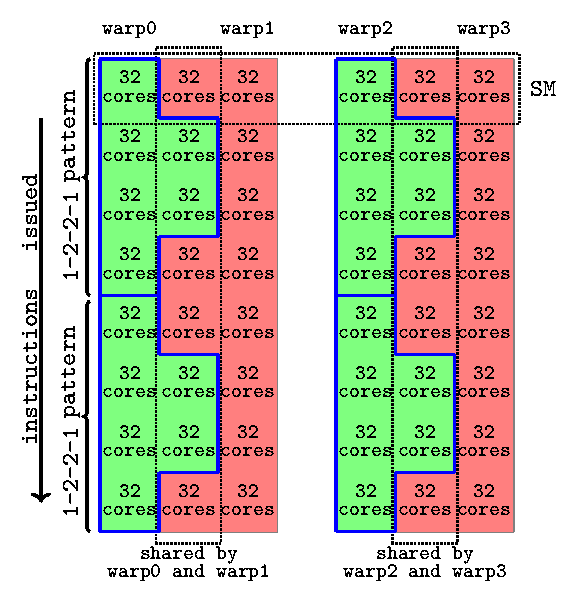
\includegraphics[scale=0.6]{warp}
    \caption{An illustration of {\tt FFMA} dual issue on one SM to achieve peak throughput}
\label{fig:warp}
\end{center}
\end{figure}

\begin{table}[htbp]
\caption{Floating-point instruction throughput on Kepler}
\centering
\scalebox{0.9} {
\begin{tabular}{|c|c|c|c|}
\hline
Inst &operation&single issue&dual issue\\
\hline
{\tt FFMA} &c=a*b+c&127.52&190.35 \\
\hline
{\tt FMUL} &c=a*b&127.52&190.35 \\
\hline
{\tt FADD} &c=a+b&127.52&191.50\\
\hline
\end{tabular}
}
\label{tab:ffma}
\end{table}

{\em {\bf Observation 4--[Memory]}: For high memory bandwidth, shared memory prefers the $64$-bit load
instruction {\tt LDS.64} while global memory prefers the $128$-bit load instruction with texture cache {\tt LDG.128}.}

For GPU memory hierarchy we focus on the programmer-controllable memory resources, shared memory and global memory.
Different memory access widths (32-, 64-, or 128-bit) and paths (through L2 cache or texture cache) exist on NVIDIA GPUs.
NVIDIA official documents and previous studies~\cite{tan} pointed out that wider
instructions have longer pipeline latency.
Our benchmarking confirms this phenomenon and also identifies several bandwidth issues for memory optimization.

Intuitively, a wider load operation should achieve higher bandwidth.
We test the bandwidth of shared memory instructions with different widths, i.e. {\tt LDS.32}, {\tt LDS.64}, and {\tt LDS.128}.
The instructions are arranged to avoid shared memory bank conflicts.
% In this experiment, the amount of data are projected to the number of load instructions.
%Assume the data can be loaded by $4N$ {\tt LDS.32} instructions,
%then $2N$ {\tt LDS.64} or $4N$ {\tt LDS.32} instructions are needed.
Figure~\ref{fig:lds_bw} compares the sequential memory access bandwidth of the three instructions by increasing the data volume.
{\tt LDS.64} achieves the highest bandwidth $137$GB/s, which is about $76\%$ of the peak shared memory bandwidth\footnote{The
theoretical shared memory bandwidth for an SM is calculated as Bandwidth = $f_{core} \times$ Width $\times$ Warpsize in bytes, where $f_{core}$ is the CUDA core frequency, Width is the bank width, Warpsize is the warp size.}.

% global memory
Two paths are used to load data from global memory, through L2 cache by {\tt
LD} instruction or texture cache by {\tt LDG} instruction.
We launch $26$ thread blocks each with $512$ threads, and specify that each thread accesses four words in a stride of $4 \times blockDim.x \times gridDim.x$.
The total accessed global memory is $256$MB.
We benchmark that a {\tt LDG.128} achieves $131$GB/s, while {\tt LD.128} only achieves $76$GB/s.
%Our benchmark confirms that {\tt LDG} achieves higher bandwidth than {\tt LD}.
% , which has been identified by previous work~\cite{tan}.

\begin{figure}[htbp]
\begin{center}
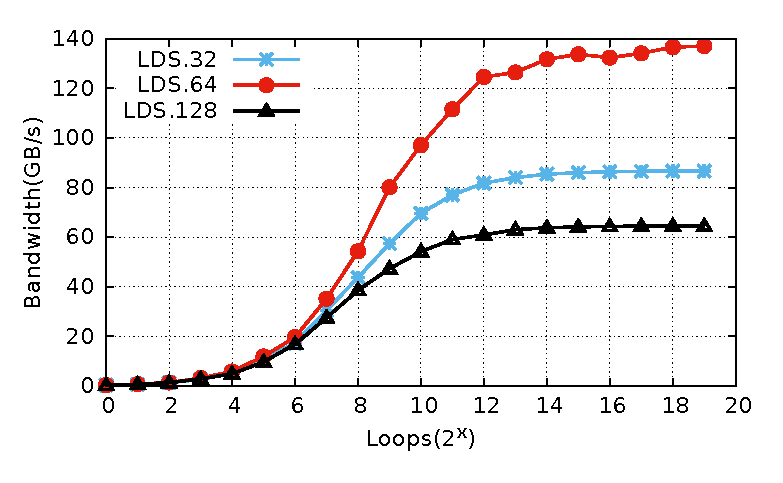
\includegraphics[scale=0.5]{lds_bandwidth}
    \caption{ The bandwidth of {\tt LDS.32}, {\tt LDS.64} and {\tt LDS.128}}
\label{fig:lds_bw}
\end{center}
\end{figure}
